%\title{Examen 1 - QuantumSeeds}

\section{Problemas Teóricos}

\subsection{Álgebra lineal}

\paragraph{A} Pruebe que dos autovectores de un operador hermitiano con diferentes eigenvalores son necesariamente ortogonales.
\subparagraph{solution}
	Sea $A$ un operador hermitiano con dos autovalores $\lambda_1$ y $\lambda_2$ distintos.
	Sea $v_{1}$ un autovector del autovalor $\lambda_1$ y $v_{2}$ un autovector del autovalor $\lambda_2$.
	Los autovalores de un operador hermitiano ($A=A^\dagger$) son reales ($\lambda=\lambda^*$) y como por definición $\braket{v_1}{Av_2}=\braket{A^\dagger v_1}{v_2}$ se tiene que
	\begin{equation*}
		\begin{split}
		\braket{v_1}{Av_2}=\braket{A v_1}{v_2}&\so\braket{v_1}{\lambda_2 v_2}=\braket{\lambda_1 v_1}{v_2}\so \\
		\lambda_2\braket{v_1}{v_2}=\lambda_1^* \braket{v_1}{v_2}&\so\lambda_2\braket{v_1}{v_2}=\lambda_1 \braket{v_1}{v_2}
		\end{split}
	\end{equation*}

Como $\lambda_1\neq\lambda_2$ la última igualdad se cumple sí y solo sí $\braket{v_1}{v_2}=0$.

\paragraph{B} Supongamos que $A$ es un operador lineal $A: V\longrightarrow W$, y $B$ es un operador lineal $B : W \longrightarrow X$.
Sean $\ket{v_i}$, $\ket{w_j}$, y $\ket{x_k}$ bases para los espacios vectoriales $V$, $W$ y $X$, respectivamente.
Muestra que la representación matricial para el operador lineal $BA$ es el producto matricial de las representaciones matriciales para B y A, con respecto a las bases apropiadas.
\subparagraph{solution}
	Sea $M$ la representación matricial de $A$ con respecto a las bases $\ket{v_i}$ y $\ket{w_j}$.
	Esto quiere decir que $A(\ket{v_i})=\sum_{j} M_{ij}\ket{w_j}$.
	Sea $N$ la representación matricial de $B$ con respecto a las bases $\ket{w_j}$ y $\ket{x_k}$.
	Esto quiere decir que $B(\ket{w_j})=\sum_{k} N_{jk}\ket{x_k}$.

	Para ver como se representa matricialmente la transformación $BA$ con respecto las bases $\ket{v_i}$ y $\ket{x_k}$, tenemos que
	\begin{equation*}
		\begin{split}
			BA(\ket{v_i})&=B(A(\ket{v_i}))=B\left(\sum_{j} M_{ij}\ket{w_j}\right)=\sum_{j} M_{ij}B(\ket{w_j})= \\
			&=\sum_{j} M_{ij}\sum_{k} N_{jk}\ket{x_k}=
			\sum_{k} \left(\sum_{j} M_{ij} N_{jk}\right)\ket{x_k}=\\
			&=\sum_{k} (MN)_{ik}\ket{x_k}
		\end{split}
	\end{equation*}


\subsection{Representación en la Esfera de Bloch de un Qubit}
Considera un qubit en un estado arbitrario $\ket{\psi}=\alpha\ket{0}+\beta\ket{1}$, donde $\alpha$ y $\beta$ son
números complejos y $|\alpha|^2 + |\beta|^2 = 1$.

\paragraph{A} Demuestra que la norma de $\ket{\psi}$ es 1, es decir, $\braket{\psi}{\psi} = 1$, utilizando la
condición de normalización de los coeficientes $\alpha$ y $\beta$.
\subparagraph{solution}
	\begin{equation*}
		\braket{\psi}{\psi}=(\alpha^*, \beta^*)\left(\begin{matrix}\alpha\\ \beta\end{matrix}\right) = \alpha^*\alpha + \beta^*\beta = |\alpha|^2 + |\beta|^2 = 1.
	\end{equation*}

\paragraph{B} Introduce las coordenadas esféricas para los coeficientes $\alpha$ y $\beta$.
\subparagraph{solution}
	Si usamos coordenadas polares y la notación de Euler, podemos encontrar número reales $r, s\geq 0$ y $\theta, \sigma\in [0,2\pi)$ tal que $\alpha=re^{i\theta}$ y $\beta=se^{i\sigma}$ con $r^2 + s^2 = 1$.

	Por otra parte, al estar $r$ y $s$ sobre una circunferencia, tenemos que existe un valor real $\phi\in [0,2\pi)$ tal que $r=\cos(\phi)$ y $s=\sin(\phi)$, así que podemos expresar los coeficientes en términos de coordenadas esféricas como $\alpha=\cos(\phi)e^{i\theta}$ y $\beta=\sin(\phi)e^{i\sigma}$.

\paragraph{C} Sustituye estas expresiones en el estado $\ket{\psi}$ y muestra cómo se puede expresar $\ket{\psi}$ en términos de los ángulos $\theta$ y $\phi$ en la esfera de Bloch.\ Donde $\theta$ y $\phi$ son ángulos esféricos.\ Es decir, que cualquier estado $\ket{\psi}$ puede representarse de manera única en la esfera de Bloch mediante estas coordenadas.

\subparagraph{solution}
	Si substituimos en la expresión de un qubit los coeficientes esféricos podemos expresar un qubit en términos de estos nuevos valores como $\ket{\psi}=\cos(\phi)e^{i\theta}\ket{0}+\sin(\phi)e^{i\sigma}\ket{1}$ que es equivalente al diferenciarse por una fase global a $\ket{\psi}=\cos(\phi)\ket{0}+\sin(\phi)e^{i(\sigma-\theta)}\ket{1}$.

	Así pues para un qubit $\ket{\psi}$ existen dos valores reales $\theta$ y $\phi$ tal que
	\begin{equation*}
		\ket{\psi}=\cos(\phi)\ket{0}+\sin(\phi)e^{i\sigma}\ket{1}
	\end{equation*}

	Estos valores representan ángulos y por la condición de normalización del qubit, nos permite representar un qubit como un elemento de una esfera de radio 1 (Esfera de Bloch) y donde $\theta$ y $\phi$ se llaman los ángulos esféricos.


\paragraph{D} Explica físicamente el significado de los ángulos $\theta$ y $\phi$ en términos de la representación en la esfera de Bloch.\ ¿Cómo se relacionan con las probabilidades de medición en las bases computacionales $\ket{0}$ y $\ket{1}$?

\subparagraph{solution}
	Por convenio, la esfera de Bloch (figura 1) se dibuja la esfera sobre los tres ejes espaciales X, Y, Z de tal modo que el ecuador quede en el plano XY.
	Los kets de la base canónica se sitúan sobre el eje Z, estando el ket $\ket{0}$ en el eje positivo y el ket $\ket{1}$ sobre el eje negativo.
	\begin{figure}[h]
		\centering
		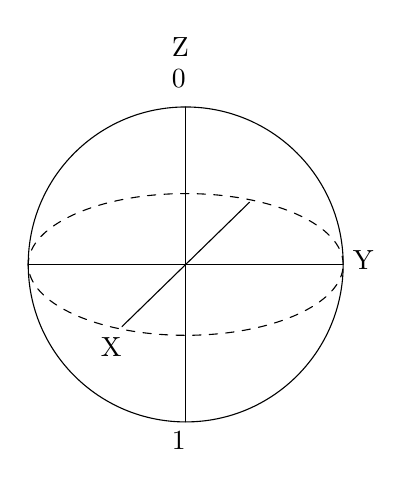
\begin{tikzpicture}
		[line cap=round, line join=round]
			\draw (0,0) circle (2cm);
			\draw [rotate around={0.:(0.,0.)},dash pattern=on 3pt off 3pt] (0,0) ellipse (2cm and 0.9cm);
			\draw (0,0) -- (0,2);
			\draw (0,0) -- (0,-2);
			\draw (0,0) -- (2,0);
			\draw (0,0) -- (-2,0);
			\draw (0,0) -- (-0.81,-0.79);
			\draw (0,0) -- (0.81,0.79);
			\draw (-0.3,3) node[anchor=north west] {Z};
			\draw (-0.3,2.6) node[anchor=north west] {$\ket{0}$};
			\draw (-0.3,-2) node[anchor=north west] {$\ket{1}$};
			\draw (2,0.3) node[anchor=north west] {Y};
			\draw (-1.2,-0.8) node[anchor=north west] {X};
		\end{tikzpicture}
		\caption{Ejes espaciales y representación de la base canónica computacional en la esfera de Bloch}
	\end{figure}

	De esta manera un qubit arbitrario se representa a través de los ángulos que forman en el ecuador entre los ejes $X$ e $Y$ y el ángulo que forma el eje $Z$ con el plano $XY$ como podemos ver en la figura 2.
	\begin{figure}[h]
		\centering
		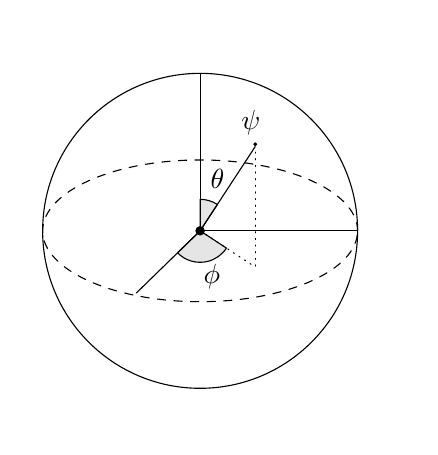
\begin{tikzpicture}
		[line cap=round, line join=round]
			\clip (-2.19,-2.49) rectangle (2.66,2.58);
			\draw [shift={(0,0)}, fill, fill opacity=0.1] (0,0) -- (56.7:0.4) arc (56.7:90.:0.4) -- cycle;
			\draw [shift={(0,0)}, fill, fill opacity=0.1] (0,0) -- (-135.7:0.4) arc (-135.7:-33.2:0.4) -- cycle;
			\draw (0,0) circle (2cm);
			\draw [rotate around={0.:(0.,0.)},dash pattern=on 3pt off 3pt] (0,0) ellipse (2cm and 0.9cm);
			\draw (0,0)-- (0.70,1.07);
			\draw (0,0) -- (0,2);
			\draw (0,0) -- (-0.81,-0.79);
			\draw (0,0) -- (2,0);
			\draw [dotted] (0.7,1) -- (0.7,-0.46);
			\draw [dotted] (0,0) -- (0.7,-0.46);
			\draw (-0.08,-0.3) node[anchor=north west] {$\phi$};
			\draw (0.01,0.9) node[anchor=north west] {$\theta$};
			\draw (0.4,1.65) node[anchor=north west] {$\ket{\psi}$};
			\scriptsize
			\draw [fill] (0,0) circle (1.5pt);
			\draw [fill] (0.7,1.1) circle (0.5pt);
		\end{tikzpicture}
		\caption{Representación de un ket $\ket{\psi}$ en la esfera de Bloch}
	\end{figure}


\section{Problema Práctico}
\subsection{Un Qubit}
Un qubit con una función de onda dada por $\ket{\psi} = (\frac{1}{2}+\frac{i}{2})\ket{0} + (\frac{1}{2}-\frac{i}{2})\ket{1}$.

\paragraph{A} Determina el bra $\bra{\psi}$ correspondiente a este estado.
\subparagraph{solution}
	Por definición $\bra{\psi}=\ket{\psi}^\dagger$, así que
	\begin{equation*}
	\bra{\psi} = (\frac{1}{2}+\frac{i}{2})^*\bra{0} + (\frac{1}{2}-\frac{i}{2})^*\bra{1} = (\frac{1}{2}-\frac{i}{2})\bra{0} + (\frac{1}{2}+\frac{i}{2})\bra{1}.
	\end{equation*}


\paragraph{B} Muestra que este estado es una función de onda normalizada, es decir, muestra que $\braket{\psi}{\psi}= 1$.
\subparagraph{solution}
	\[
		\braket{\psi}{\psi} = (\frac{1}{2}+\frac{i}{2})^* (\frac{1}{2}+\frac{i}{2}) + (\frac{1}{2}-\frac{i}{2})^* (\frac{1}{2}-\frac{i}{2})=\frac{1}{4}+\frac{1}{4}+\frac{1}{4}+\frac{1}{4}=1.
		\]

\paragraph{C} Si se mide este qubit en la base computacional $\set{\ket{0}, \ket{1}}$, ¿cuáles son las
probabilidades de obtener cada uno de los dos resultados para esta medición?
\subparagraph{solution}
	La probabilidad de obtener el valor $0$ al medir es el cuadrado del coeficiente, es decir $(\frac{1}{2}+\frac{i}{2})^* (\frac{1}{2}+\frac{i}{2})=\frac{1}{2}$, y análogamente la probabilidad de obtener $1$ es $(\frac{1}{2}-\frac{i}{2})^* (\frac{1}{2}-\frac{i}{2})=\frac{1}{2}$.


\paragraph{D} Define los dos estados de base $\ket{+}=\frac{1}{\sqrt{2}}\ket{0}+\frac{1}{\sqrt{2}}\ket{1}$ y $\ket{-}=\frac{1}{\sqrt{2}}\ket{0}-\frac{1}{\sqrt{2}}\ket{1}$.
Calcula el producto interno de estos estados con $\ket{\psi}$.
Es decir, encuentra $\braket{+}{\psi}$ y $\braket{-}{\psi}$.
\subparagraph{solution}
	\begin{equation*}
		\begin{split}
			\braket{+}{\psi} &= \frac{1}{\sqrt{2}}\left(\frac{1}{2}+\frac{i}{2}\right)+\frac{1}{\sqrt{2}}\left(\frac{1}{2}-\frac{i}{2}\right)= \frac{1}{\sqrt{2}}\\
			\braket{-}{\psi} &= \frac{1}{\sqrt{2}}\left(\frac{1}{2}+\frac{i}{2}\right)-\frac{1}{\sqrt{2}}\left(\frac{1}{2}-\frac{i}{2}\right)= \frac{i}{\sqrt{2}}\\
		\end{split}
	\end{equation*}


\paragraph{E} Verifica que $\ket{+}$ y $\ket{-}$ son ortogonales: $\braket{+}{-}= 0$.
Asegúrate también de que $\ket{+}$ y $\ket{-}$ estén normalizados correctamente.
En otras palabras, muestra que $\braket{+}{+}=\braket{-}{-}=1$.
\subparagraph{solution}
	\begin{equation*}
		\begin{split}
			\braket{+}{+} &= \frac{1}{\sqrt{2}}\frac{1}{\sqrt{2}}+\frac{1}{\sqrt{2}}\frac{1}{\sqrt{2}}=1\\
			\braket{-}{-} &= \frac{1}{\sqrt{2}}\frac{1}{\sqrt{2}}+\frac{-1}{\sqrt{2}}\frac{-1}{\sqrt{2}}=1\\
			\braket{+}{-} &= \frac{1}{\sqrt{2}}\frac{1}{\sqrt{2}}+\frac{1}{\sqrt{2}}\frac{-1}{\sqrt{2}}=0\\
		\end{split}
	\end{equation*}


\subsection{Estados Bell y Matrices de Densidad}
Considera el estado de Bell $\ket{\psi}_{AB}=\frac{1}{\sqrt{2}}(\ket{01}+\ket{10})$.

\paragraph{A} ¿Cuál es la matriz de densidad $\rho_{AB}$ para el sistema completo de 2 qubits?
\subparagraph{solution}
	Para un estado puro la matriz de desidad es $\rho_{AB}=\ketbra{\psi}{\psi}$.
	\begin{equation*}
		\begin{split}
		\rho_{AB}&=\ketbra{\psi}{\psi}=\frac{1}{2}\ketbra{01}{01}+\frac{1}{2}\ketbra{01}{10}+\frac{1}{2}\ketbra{10}{01}+\frac{1}{2}\ketbra{10}{10}=\\
		&=\begin{pmatrix}
		0 & 0 & 0 & 0 \\ 0 & \frac{1}{2} & \frac{1}{2} & 0 \\ 0 & \frac{1}{2} & \frac{1}{2} & 0 \\ 0 & 0 & 0 & 0 \end{pmatrix}.
		\end{split}
	\end{equation*}


\paragraph{B} Calcula la matriz de densidad $\rho_A = \Tr_B(\rho_{AB})$.
\subparagraph{solution}
Por definición los elementos de $\rho_A$ son
	\begin{equation*}
\begin{split}
		(\rho_A)_{ij}&=\sum_{k=0}^1 \mel{ik}{\rho_{AB}}{jk}\\
		(\rho_A)_{00}&=\mel{00}{\rho_{AB}}{00}+\mel{01}{\rho_{AB}}{01}=\frac{1}{2}\\
		(\rho_A)_{01}&=\mel{00}{\rho_{AB}}{10}+\mel{01}{\rho_{AB}}{11}=0\\
		(\rho_A)_{10}&=\mel{10}{\rho_{AB}}{00}+\mel{11}{\rho_{AB}}{01}=0\\
		(\rho_A)_{11}&=\mel{10}{\rho_{AB}}{10}+\mel{01}{\rho_{AB}}{11}=\frac{1}{2}\\
\end{split}
	\end{equation*}
	Entonces $\rho_{A}=\begin{pmatrix}\frac{1}{2} & 0 \\ 0 & \frac{1}{2} \end{pmatrix}$.

\paragraph{C} Calcula la matriz de densidad $\rho_B = \Tr_A(\rho_{AB})$.

\subparagraph{Solution}
	Análogamente para la matriz $\rho_B=\sum_{k=0}^1 \mel{ki}{\rho_{AB}}{kj}$ al hacer la cuentas como en el apartado B se obtiene la misma matriz,
\[
	\rho_{B}=\begin{pmatrix}\frac{1}{2} & 0 \\ 0 & \frac{1}{2} \end{pmatrix}.
\]


\paragraph{D} Se utiliza el estado $\ket{\psi}_{AB}$ como recurso en un protocolo cuántico de comunicación.
Explica cómo la matriz de densidad reducida $\rho_A$ del primer qubit puede proporcionar información sobre la información cuántica accesible para un observador que tiene acceso solo al primer qubit.
¿Cómo influye esto en la capacidad de transmitir información cuántica de manera segura y eficiente utilizando este estado Bell en un protocolo de comunicación cuántica?

\section{Problema Computacional}
\subsection{Qubits y Compuertas en Qiskit}
Considere un sistema cuántico de un solo qubit inicializado en el estado $\ket{-}$.
Utilizando Qiskit, resuelva las siguientes tareas:

\paragraph{A} Implemente una secuencia de compuertas cuánticas en Qiskit para transformar el estado del qubit según la siguiente operación:
\[
U = X  H  Z
\]
Donde:
\begin{itemize}
\item X es la compuerta de Pauli-X,
\item H es la compuerta de Hadamard,
\item Z es la compuerta de Pauli-Z.
\end{itemize}

\subparagraph{solution}

	\begin{verbatim}
	from qiskit import QuantumCircuit
	circuit = QuantumCircuit(1)
	circuit.x(0)
	circuit.h(0)
	circuit.z(0)
	\end{verbatim}


\paragraph{B} Expresa la matriz unitaria asociada con la secuencia de compuertas $U$.
\subparagraph{solution}
	\begin{verbatim}
	from qiskit.quantum_info import Operator
  matrix = Operator(circuit)
  array_to_latex(matrix)
	\end{verbatim}
	\[
		\text{matrix} = \begin{pmatrix}\frac{\sqrt{2}}{2} & \frac{\sqrt{2}}{2} \\ \frac{\sqrt{2}}{2} & \frac{-\sqrt{2}}{2}
		\end{pmatrix}
	\]


\paragraph{C} Aplique la secuencia de compuertas U al estado inicial del qubit y calcule el nuevo estado resultante del sistema.
\subparagraph{solution}
	\begin{verbatim}
		from qiskit import execute
from qiskit.providers.aer import StatevectorSimulator
backend = StatevectorSimulator()
initialState = QuantumCircuit(1)
initialState.x(0)
initialState.h(0)
finalState = initialState.compose(circuit)
job = execute(finalState, backend)
job_result = job.result()
print(job_result.get_statevector(finalState, decimals=3))
	\end{verbatim}
	\[
			\text{finalState} = ([-0.+0.j,  1.+0.j], dims=(2))
	\]


\paragraph{D} Expresa este nuevo estado como un vector de estado.
\subparagraph{solution}
	\[
			\text{finalState} = \ket{1}
	\]

